\documentclass[a4paper, 12pt]{article}

\usepackage{geometry}
\geometry{a4paper,
total={170mm,257mm},left=2cm,right=2cm,
top=1cm,bottom=2cm}
\usepackage{wrapfig}
\usepackage{graphicx}
\usepackage{mathtext}
\usepackage{amsmath}
\usepackage{siunitx} % Required for alignment
\usepackage{multirow}
\usepackage{gensymb}
\usepackage{rotating}
\sisetup{
  round-mode          = places, % Rounds numbers
  round-precision     = 2, % to 2 places
}

\usepackage[T1,T2A]{fontenc}

\usepackage[russian]{babel}

\graphicspath{{pictures/}}


\title{\begin{center}Лабораторная работа №2.1.3\end{center}
Определение \(C_p/C_v\) по скорости звука в газе.}
\author{Каграманян Артемий, группа Б01-208}
\date{\today}

\begin{document}

\maketitle

\section{Аннотация}

\textbf{Цель работы:} 1) Измерение частоты колебаний и длины волны при резонансе звуковых колебаний в газе, заполняющем трубу. 2) Определение показателя адиабаты с помощью уравнения состояния идеального газа.

\textbf{Оборудование:} Звуковой генератор, осцилограф, изолированная труба, термостат.

\section{Теоритическая справка}
Как нам известно, скорость звука определяется такой формулой:
\begin{equation}
  c = \sqrt{\gamma \frac{RT}{\mu}}
\end{equation}

Немного преобразуем формулу:
\begin{equation}
  \gamma = \frac{\mu}{RT}c^2
\end{equation}

Звуковыя волна многократно отражается от стенок трубы. Если мы зададим длину волны так, что выполняется выражение (3), то амплитуда колебаний резко увеличится, и наступит резонанс:
\begin{equation}
  L = \frac{\lambda}{2}n
\end{equation}
В этом случае конец волны совпадет с началом, и эта волна совпадет по фазе с предыдущей. Совпадающие по фазе волны усиливают друг друга. Поэтому наступает резонанс. \\
Так же мы можем найти скорость звука как \(c = f \lambda\). \\

\section{Методика эксперимента}
В данной работе резонансы производятся следующим образом: для фиксированной длины \(L\) трубы подбираются 8 частот звуковых волн, для которых выполняется слеующее:
\begin{equation}
  L = \frac{\lambda_{1}}{2}n_1 = \cdots = \frac{\lambda_{i}}{2}n_i = \cdots = \frac{\lambda_{8}}{2}n_8 
\end{equation}
Подставив $\lambda = \frac{c}{f}$, получим:
\begin{equation}
  f = \frac{c}{2L}n
\end{equation}
Этот процесс производим для каждой рассматриваемой температуры. Затем строим графики, на которых отобразим по оси \(x\) значение \(n_i\), а по оси \(y\) значение \(f_{i + 1} - f_1\).
Таким образом, мы, построив аппроксиммирующие прямые, получим величину \(c/2L\), и отсюда найдем скорость звука при данной температуре.

\section{Экспериментальная установка}

\begin{figure}[h]
  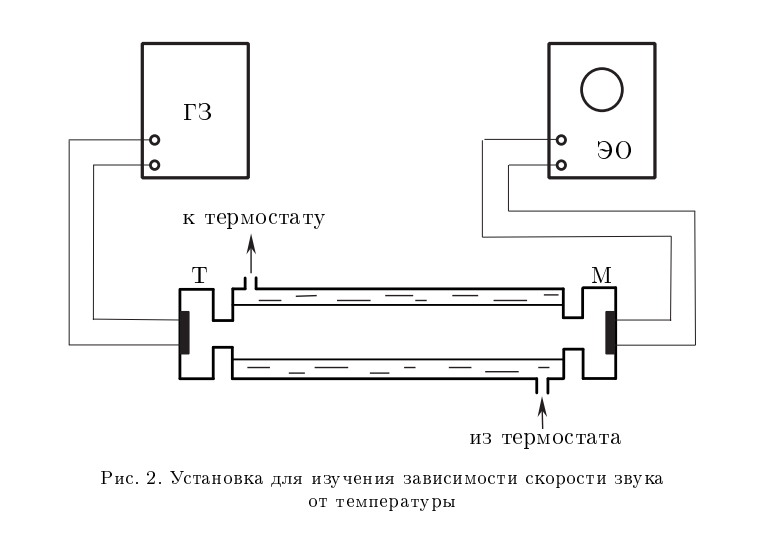
\includegraphics[width = 1\linewidth]{ust.png}
\end{figure}

\newpage
\section{Обработка данных}
Итого, у меня получились следующие значения для резонансов:
\begin{table}[h]
  \begin{center}
  \begin{tabular}{|c|c|c|c|c|c|c|c|c|}
    \hline
    T, К & $f_1$ & $f_2$ & $f_3$ & $f_4$ & $f_5$ & $f_6$ & $f_7$ & $f_8$ \\
    \hline
    296,10 & 210,3 & 440,2 & 710,4 & 935,3  & 1190,3 & 1405,3 & 1710,1 & 1853,9 \\
    323    & 231,1 & 484,7 & 732,7 & 975,3  & 1225,1 & 1454,8 & 1720,6 & 1917,6 \\
    338    & 244,1 & 496,8 & 745,7 & 992,7  & 1228,1 & 1471,3 & 1733,6 & 1987,2 \\
    353    & 258,3 & 515,6 & 755,8 & 1017,0 & 1255,6 & 1508,4 & 1759,3 & 2018,2 \\
    \hline
  \end{tabular}
  \end{center}
\end{table}

Итого, получился график ($k = \frac{c}{2L}$):
\begin{figure}[h]
  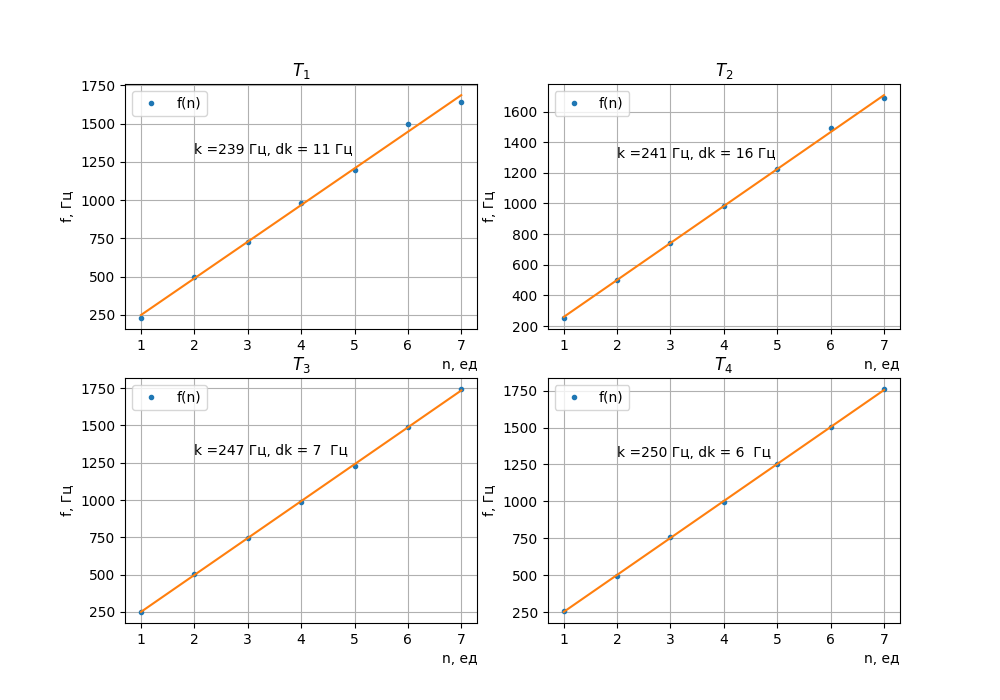
\includegraphics[width = 1\linewidth]{plot.png}
\end{figure}

Итого, получается, что:
\begin{table}[h]
  \begin{center}
  \begin{tabular}{|c|c|c|c|c|}
    \hline
    с, $\frac{м}{с}$ & 273,3 & 275,8 & 278,7 & 280,0 \\
    \hline
    $\Delta$ c, $\frac{м}{с}$  & 0,8 & 0,9 & 0,5 & 0,5  \\
    \hline
    $\gamma$ & 1,27 & 1,29 & 1,32 & 1,33 \\
    \hline
  \end{tabular}
  \end{center}
\end{table}

\section{Вывод}
Мы получили $\gamma$ близкое к табличным (табличное - 1.3). Погрешность получилась из-за неточного снятия данных с осцилографа.
\end{document}